\documentclass[10pt,conference,letterpaper]{IEEEtran}
\usepackage{verbatim}
\usepackage{moreverb}
\usepackage{url}
\usepackage{amsmath}
\usepackage{color}

\title{HAMAKE: A Dataflow Approach to Data Processing in Hadoop}

\author{\IEEEauthorblockN{Vadim Zaliva}
\IEEEauthorblockA{Codeminders\\
Email: lord@crocodile.org} \and \IEEEauthorblockN{Vladimir Orlov}
\IEEEauthorblockA{Codeminders\\
Email: vorl@codeminders.com}}

\date{2011}
\usepackage{graphicx}
\usepackage{listings}
\usepackage{rotating}
\usepackage[colorlinks=false,bookmarks=true,pdfauthor={Vadim Zaliva lord@crocodile.org, Vladimir Orlov vorl@codeminders.com},
            pdftitle={HAMAKE: A Dataflow Approach to Data Processing in Hadoop},
            pdftex]{hyperref}

% graphviz.tex
% originally written by Derek Rayside, November 2003
% following an idea that Daniel Jackson implemented in his Tagger program
%
% parameters to \digraph:
% 1 - parameters for \includegraphics (optional; default value is "scale=1")
% 2 - name of the digraph
% 3 - body of the digraph

\newcommand{\digraph}[3][scale=1]{
    \newwrite\dotfile
    \immediate\openout\dotfile=#2.dot
    \immediate\write\dotfile{digraph #2 {\string#3}}
    \immediate\closeout\dotfile
    \IfFileExists{#2.ps}
        % the postscript exists: include it
        { \includegraphics[#1]{#2} }
        % the postscript doesn't exist: tell the user how to create it
        { \fbox{ \begin{tabular}{l}
            The file \texttt{#2.ps} hasn't been created from
            \texttt{#2.dot} yet. \\
            Run `\texttt{dot -Tps -o #2.ps #2.dot}' to create it. \\
            Here is a \textsf{bash} loop to process all \textsf{dot} files
            in the current directory: \\
            \texttt{
            for f in *.dot do ; 
            dot -Tps -o \$\{f\%dot\}ps \$f ; 
            done
            }
            \end{tabular}}
        }
}


\begin{document}
\lstset{language=XML,basicstyle=\tiny,markfirstintag=true,numbers=left,numbersep=1pt}

\maketitle

\begin{abstract}
  Most non-trivial data processing scenarios using Hadoop typically
  involve launching more than one MapReduce job. Usually, such
  processing is data-driven, with the data funneled through a sequence
  of jobs. The processing model could be expressed in terms of
  dataflow programming.
  
  It could be represented as a directed graph, with datasets as
  vertices. Using \textit{fuzzy timestamps} as a way to detect which
  dataset needs to be updated, we can calculate a sequence in which
  Hadoop jobs need to be launched to bring all datasets up to
  date. Incremental data processing and parallel job execution fit
  well into this approach.

  These ideas inspired the creation of \textbf{hamake} utility. We
  attempted to emphasize data and allowing the developer to formulate
  his or her problem as a data flow (opposed to a workflow approach
  commonly used). \textbf{hamake} language using just two data flow
  operators: \emph{fold} and \emph{foreach} providing a clear
  processing model, similar to MapReduce, but on a dataset level.
\end{abstract}

\section{Motivation and History}

MapReduce data processing model have been introduced by
Google\cite{dean2008map}. Hadoop\cite{bialecki2005hadoop} is popular
open-source implementation of MapReduce.

Hadoop is typically used to process big amounts of data via series of
relatively simple operations. Usually Hadoop jobs are I/O-bound
\cite{hadoopattwitter},\cite{hs2010hadoopbench}, and execution of even
trivial operation on large dataset could take significant system
resources. This makes incremental processing important. Or initial
inspiration was Unix \emph{make} utility. While applying some of ideas
implemented in it to Hadoop, we took an opportunity to generalise
processing model in terms of dataflow programming.

\textbf{hamake} was developed in late 2008 to address the problem of
incremental processing of big data sets in a collaborative filtering
project.

We've striven to create a simple to use utility that developers can
start using right away without complex installation or extensive
learning. 

\textbf{hamake} is open source, distributed under Apache
License v2.0. The project is hosted at google code at the following
URL: \url{http://code.google.com/p/hamake/}.

\section{Processing Model}

\textbf{hamake} operates on \textit{files}, residing on local or
distributed file system accessible from Hadoop job (usually it is
HDFS). Each file has a timestamp, reflecting date and time of its last
modification. A file system directory or folder is also a file, and
has its own timestamp. A \textit{Data Transformation Rule (DTR)}
defines an operation which takes files or filesets as inputs and
produce other files or filesets as outputs.

If file \textit{A} is listed as input of a DTR, and file \textit{B}
listed as output of the same DTR, it is said that \textit{``B depends
  on A''}. \textbf{hamake} is using file time stamps for dependency
up-to-date checks. DTR outputs said to be \textit{up to date} if
minimum time stamp on all its outputs is greater or equal than maximum
timestamp on all inputs. A user, for his or her convenience, could
arrange groups of files and folders into a \emph{fileset} which later
could be references as DTR's input or output.

\textbf{hamake} is using \textit{fuzzy timestamps}\footnote{Current stable
  version of \textbf{hamake} is using exact (non-fuzzy) timestamps.}
which could be compared, allowing for a certain margin or error. The
``fuzziness'' is controlled by tolerance $\sigma$. Timestamp $a$ is
considered to be older than timestamp $b$ if $(b-a)>\sigma$. Setting
$\sigma=0$ gives us non-fuzzy, strict timestamp comparison.

\textbf{hamake} attempts to ensure that all DTR outputs are up to
date\footnote{\textbf{hamake} does not try to ensure that files which are not
  listed as one of DTR outputs are up to date, because it has no way
  to update them.}.  To do so it builds a \textit{dependency
  graph}. This graph have individual files or filesets as vertices and
DTRs as edges. We will see below that this is guaranteed to be a
\textit{Direct Acyclic Graph} (DAG).

Then, a graph reduction algorithms shown on Figure~\ref{fig:grred} is
executed. It is using to Kahn's algorithm\cite{kahn1962topological},
of topological ordering.

\begin{figure}[htp]
\centering
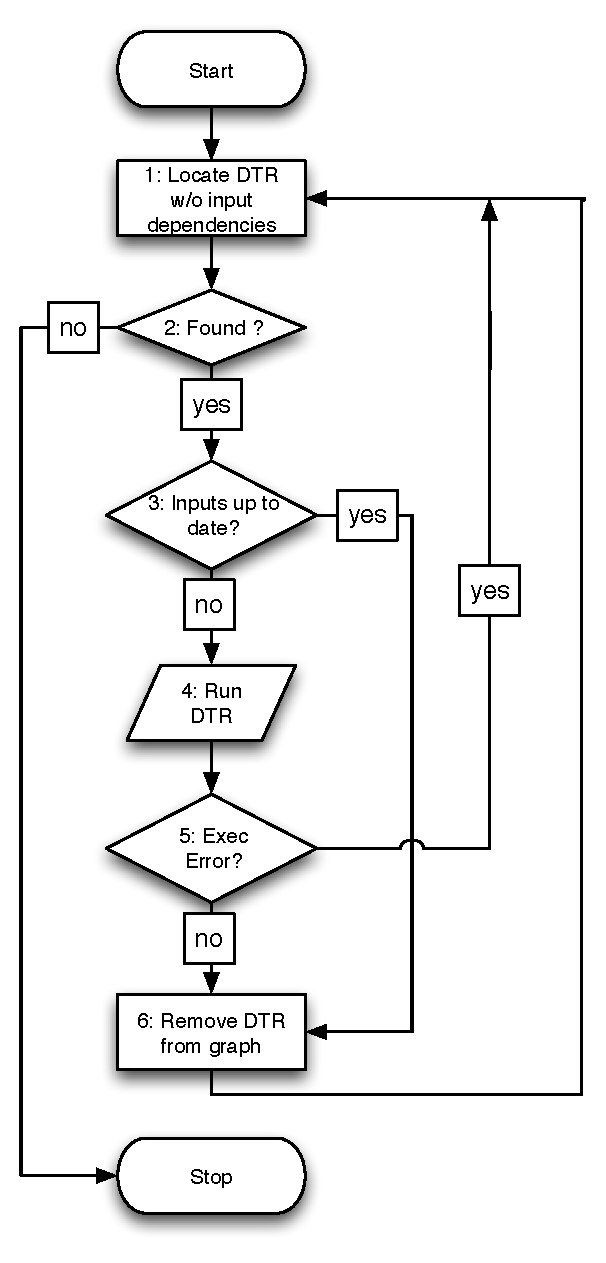
\includegraphics[width=4cm]{GraphReduction.eps}
\caption{\textbf{hamake} dependency graph reduction algorithm}
\label{fig:grred}
\end{figure}

The algorithms allows for parallelism. If more than one DTR without
input dependencies is found during step 1, subsequent steps 2-5 could
be executed for each discovered DTR in parallel.

It should be noted that if DTR exectuion has failed, \textbf{hamake} still can
and will process other DTRs which do not depend directly or indirectly
on results of this DTR. This permits user to fix the problem later and
re-run \textbf{hamake}, without need to re-process all data.

Cyclic dependencies has to be avoided, because a dataflow containing
such dependencies is not guaranteed to terminate. Implicit checks are
performed during reading DAG definitions and building dependency
graph. If a cycle is detected, it is reported as an error. So the
dependency graph used by \textbf{hamake} ensured to be a
\textit{directed acyclic graph}.

However \textbf{hamake} supports a limited scenario of iterative
processing, where DTR output of one \textbf{hamake} execution could used as
another DTR's input during the next \textbf{hamake} run. This mechanism is
implemented via \textbf{hamake} feature called
\textit{generations}. Each input or output file could be optionally
marked with \emph{generation} attribute. The two files with different
generation numbers although referencing the same path on file system
are treated as different vertex is dependency graph.

One useful consequence of \textbf{hamake} dataflow being a DAG, is
that for each vertex we can calculate list of vertices it depends on,
directly and indirectly using simple \textit{transitive closure}. On
datasets, where the cost of re-calculation could be potentially high
(due to data size or computational complexity) this allows to estimate
the scope of dataflow graph affected by updating one or more files.

\textbf{hamake} is driven by dataflow description, expressed in simple
XML-based language. The full syntax is described in
\cite{hamakesyntax}. Two main elements \emph{fold} and \emph{foreach},
corresponding to two types of DTRs. Each of them have inputs, outputs
and processing instruction. Executing processing instruction should
bring DTR outputs up to date, compared to its inputs. \emph{fold}
implies many-to-one dependency between inputs and the outputs. In
other words, outputs depends on all inputs and if either of inputs
have been changed, outputs needs to be updated. \emph{foreach} implies
one-to-one dependency: where for each file in input set there is a
corresponding output file, each of them updated independently.

\textbf{hamake} dataflow language has a declarative semantics. Keeping it
purely declarative, makes it easy in future to implement various
dataflow analysis and optimization algorithms on top of it. Some
examples of such algorithms could be: merging dataflows, further
execution parallelization, dataflow complexity analysis and
estimation.

\section{Scheduler}

\textbf{hamake} scheduler is responsible determining the sequence and
launching Hadoop jobs required to bring all datasets up-to-date.  It
attempts to perform all required computations in shortest possible
time. To achieve this it aims for maximal cluster utilization, running
as many Hadoop jobs in parallel as cluster capacity permits.

There are three main factors driving scheduling logic: file
timestamps, dependencies, and cluster computational capacity. On
highest level DTR dependencies determine sequence of DTRs jobs being
launched.

In case of \emph{fold} DTR, a single Hadoop job, PIG script or shell
could be launched and hence there are not many opportunities to for
parallel execution. In example shown on Figure~\ref{fig:fold1}, since
fileset \textit{B} depends on all files in fileset \textit{A}, a
single job associated with \emph{fold} DTR will be executed.

\begin{figure}[htp]
\centering
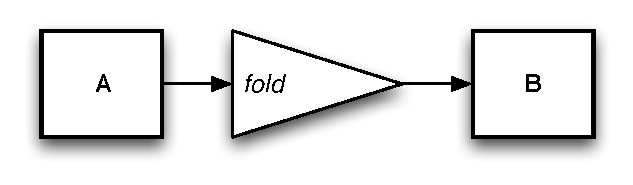
\includegraphics[width=0.3\textwidth]{twofold.eps}
\caption{Simple \emph{fold} DTR}
\label{fig:fold1}
\end{figure}

At first glance, \emph{foreach} DTR shown in Figure~\ref{fig:foreach1}
looks similar to \emph{fold}.

\begin{figure}[htp]
\centering
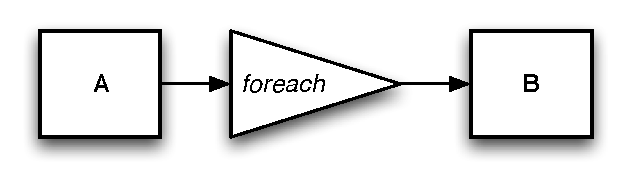
\includegraphics[width=0.3\textwidth]{twoforeach.eps}
\caption{Simple \emph{foreach} DTR}
\label{fig:foreach1}
\end{figure}

However \emph{foreach} DTRs works by mapping individual files in
fileset \textit{A} to files in fileset \textit{B}. Assuming that
fileset \textit{A} consists of 3 files: \textit{$a_1$},
\textit{$a_2$}, \textit{$a_3$} the the dependency graph could be
represented as shown on Figure~\ref{fig:foreach2}. In this case we
have an opportunity to execute three jobs in parallel.

\begin{figure}[htp]
\centering
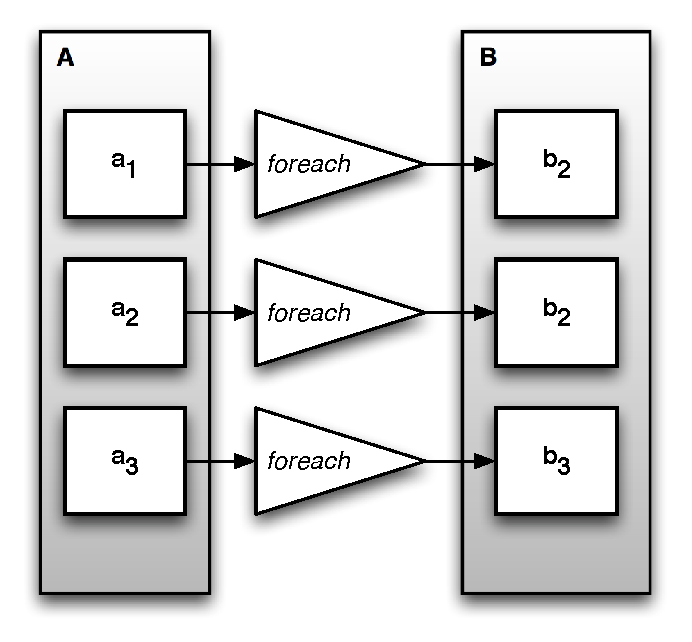
\includegraphics[width=0.3\textwidth]{twoforeachp.eps}
\caption{Decomposition of \emph{foreach} DTR}
\label{fig:foreach2}
\end{figure}

The Hadoop cluster capacity is defined in terms of number of
\textit{map slots} and \textit{reduce slots}. DTR launches Hadoop job
(either directly as defined by \emph{mapreduce} processing instruction
or via PIG script, single job will spawn one or more \emph{mapper} and
\emph{reducer} tasks, each taking one respective slot. Number of
mappers and reducers lauched depends on many factors, such as size of
HDFS block, Hadoop cluster settings, \emph{JobConf} settings. In
general, \textbf{hamake} does not have an neither visibility nor
control over most of these factors, so the \textbf{hamake} scheduler
currently does not deal with individual tasks. It knows only about
data files and spawned Hadoop jobs.

\section{Example}

Let us consider a hypothetical example, demonstrating \textbf{hamake}
use. Imagine an online library containing digital copes of millions of
books. Considering a size of such library, it's hardly surprising that
there are duplicated titles in it. Such duplicates may be caused by
OCR errors, typos, differences in formatting, or added material such
as foreword or a publisher information.

For the purpose of illustration of \textbf{hamake} usage we will
consider simple approach of using d \textit{vector space
  model}\cite{manning2008introduction} based on word frequencies and
\textit{Canopy clustering algorithm}\cite{efficientClustering}. The
implementation could be split into series of steps, each of them
represented by a \textit{MapReduce job}:

\begin{description}[\IEEEsetlabelwidth{\emph{FilterStopwords}}]
\item[\emph{ExtractText}] Extract a plain text from native document format
  (e.g. PDF or EPUB).
\item[\emph{Tokenize}] Split plain text into a tokens, roughly
  corresponding to words. Dealing with hyphens, compound words,
  accents and diacritics, case-folding, stemming or lemmatization of
  tokens, resulting in a list of normalized \text{tokens}.
\item[\emph{FilterStopwords}] Filtering out \textit{stopwords} (e.g. words
  like \textit{a}, \textit{the}, \textit{are}) from the list of
  terms.
\item[\emph{CalculateTF}] For each document calculate a feature
  vector: a vector of term frequencies.
\item[\emph{FindSimilar}] Run \textit{Canopy clustering algorithm}
  for grouping similar books in clusters. Use
  \textit{cosine distance} as a fast approximate distance metric. 
\item[\emph{OutputResult}] Output book names, which are found in
  clusters with more than 1 elements
\end{description}

Each of resulting six MapReduce jobs produces and output files which
depends on inputs. For each book, they have to be invoked
sequentially, as outputs of one tasks are used as inputs of the next
one. Additionally, there is a configuration file containing list of
stop words, and some tasks output depend on this file content. These
dependencies could be represented by direct acyclic graph, show on
Figure~\ref{fig:SimilarityAlgDAG}, with vertices representing data
files, and jobs assigned to edges. The XML file describing the
dataflow in \textbf{hamake} language is show as
Listing~\ref{hamakeFile}.

\lstinputlisting[caption={\textit{hamakefile}, that describes process for
  detecting similar books}, label=hamakeFile]{sample.xml}

The first DTR (lines 10-25) converts a book from native format such as
PDF or EPUB to plain text. The input of the DTR is a reference to to
\emph{/doc} folder, and the output is \emph{/txt} folder. The
\emph{foreach} DTR establishes one to one dependency between files
with the same names in these two folders. The Hadoop job which
performs actual text extraction is defined using \emph{mapreduce}
element. It will be invoked by \textbf{hamake} for each unsatisfied
file dependency. The job takes two parameters, defined with
\emph{parameter} elements - an input a path to a book, and a path to a
file, where plain text version should be written. The remaining five
DTRs are defined in the similar manner.

\textbf{hamake}, when launched with this XML descriptor will first
search for DTRs that has no inputs or which inputs are not outputs of
other tasks. In our particular example, this is
\emph{ExtractPlainText}. \textbf{hamake} will launch this job first,
an as soon as it will be finished, will execute jobs which depend on
outputs of this task, and so on while all files are up to date. As a
result of this data flow, you will get a file \emph{results.txt} with
list of similar books.

This data flow could be used for incremental processing. When new
books are added, \textbf{hamake} will not re-run following DTRs:
\emph{ExtractText}, \emph{Tokenize}, \emph{FilterStopWords}, and
\emph{CalculateTF} for previously processed books. However it will run
these DTRs for newly added books, and then, will re-run
\emph{FindSimilar} and \emph{OutputResults}.  If list of stop words
has been changed, \textbf{hamake} will re-run only
\emph{FilterStopWords} \emph{CalculateTF}, \emph{FindSimilar}, and
\emph{OutputResults} DTRs.

\begin{figure}[htp]
\centering
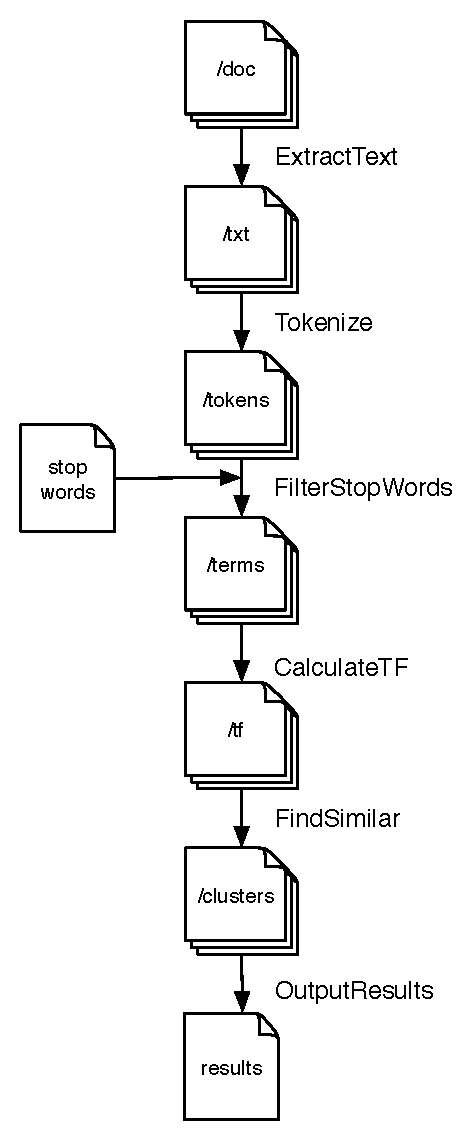
\includegraphics[width=0.25\textwidth]{SimilarityAlgDAG.eps}
\caption{Directed Acyclic Graph of a similar books detection data flow}
\label{fig:SimilarityAlgDAG}
\end{figure}

\section{Related Work}

Several workflow engines exist for Hadoop, such as
\href{http://github.com/tucu00/oozie1}{Oozie},
\href{http://sna-projects.com/azkaban/}{Azkaban}, and
\href{http://www.cascading.org/}{Cascading}.  Although all of these
products could be used to solve similar problems, they differ
significantly in design, philosophy, target user profile, usage
scenarios, etc., limiting usefulness of simple feature-wise
comparison.

The main, most significant difference between these engines and \textbf{hamake}
lies in \textit{workflow} vs. \textit{dataflow} approach. All of them
using the former, explicitly specifying dependencies between
jobs. \textbf{hamake}, on the other hand, using dependencies between datasets,
to derive the workflow. Both approaches are have their advantages. One
can argue that for some problems a dataflow representation, used by
\textbf{hamake} is more natural than a workflow.

\section{Future Work}

One of possible \textbf{hamake} improvements is a better integration with
Hadoop schedulers. For example if \textit{Capacity Scheduler} or
\textit{Fair Scheduler} is used, a \textbf{hamake} can take into account
information about its \textit{pools} or \textit{queues} capacities in
job scheduling algorithm.

Another potential area of future extension is \textbf{hamake} dependency
mechanism. Current implementation using fairly simple timestamp
comparison to check if dependency is satisfied. This could be
generalized, allowing user to specify custom dependency check
predicates, implemented either as plugins, scripts in some embedded
scripting language or external programs. This would allow to make
decisions not only based on file meta data (such as timestamp) but
also on its contents.

Several \textbf{hamake} users has requested support of iterative computations
with termination condition. Possible use-cases calling for this type
of usage are fixed-point computations, iterative regression, or
clustering algorithms. Presently, to embed this kind of algorithms
into \textbf{hamake} work flow require use of \textit{generations} feature
combined with external automation, invoking \textbf{hamake} repeatedly until
certain exit condition it satisfied. \textbf{hamake} users could
certainly benefit from native support for this kind of dataflows by
\textbf{hamake}.

\nocite{*}
\bibliography{hamake}
\bibliographystyle{unsrt}

\end{document}
